\documentclass[coverpage]{article}

\usepackage[affil-it]{authblk}
\usepackage[margin=1in]{geometry}
\usepackage{pdfpages}
\usepackage{subcaption}
\usepackage{amsmath}
\usepackage{url}
\usepackage{fancyhdr}
	\fancyfoot{}
	\lhead{Mermelstein, \thepage}
	\pagestyle{fancy}

\newcommand{\softwareText}[1]{\textit{#1}\texttrademark}
\newcommand{\loggerpro}{\softwareText{Logger Pro}}
\newcommand{\origin}{\softwareText{Origin Pro}}
\newcommand{\iUnit}{\text{kg $\text{m}^2$}}
\newcommand{\rwheel}{Roto-Dyne wheel}
\newcommand{\mpssq}{\frac{\text{m}}{\text{s}^2}}

\title{Rotational Kinetic Energy Lab}
\date{October 31, 2023}
\author{Wolf S. Mermelstein}
\affil{Department of Physics, Case Western Reserve University, Cleveland, Ohio, 44106-7079}

\begin{document}
	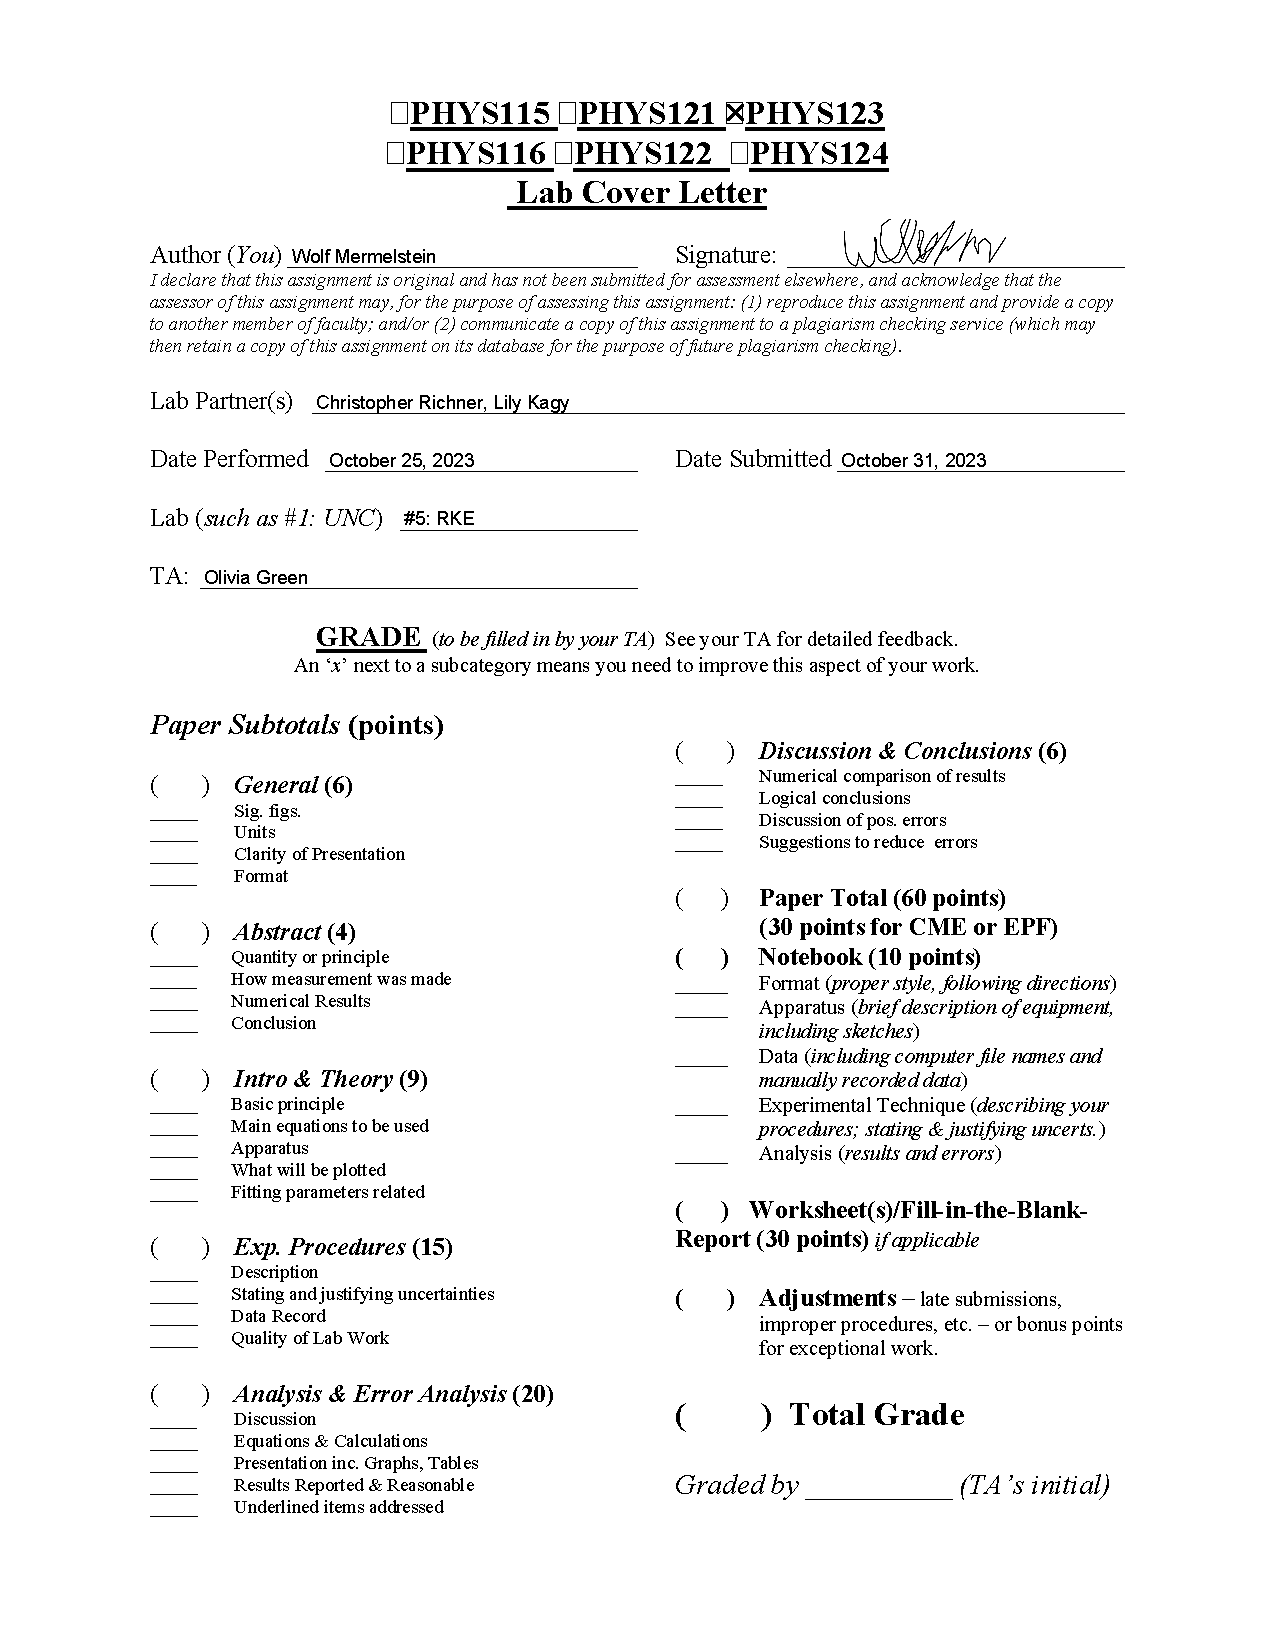
\includepdf{reportCover.pdf}
	
	\maketitle
	
	\begin{abstract}
		Our experiment studied the law of conservation of energy by using it to experimentally determine the moment of inertia of a \rwheel. We attempted to guess a reasonable value based on similar shapes, such as a disc and ring, and then performed a Monte Carlo simulation to apply some degree of uncertainty to our estimate. The Monte Carlo simulation estimate for $I$, which we call $I_M$, was $0.07182 \pm 0.00104\ \iUnit$. We then experimentally measured the moment of inertia for the system, and determined that $I$, which we called $I_1$ for the given system, was $0.06663 \pm 0.00017 \iUnit$. Using this information we finally attempted to find the specific moment of inertia for load masses discluding the \rwheel. To do this we also experimentally measured the moment of inertia of the \rwheel~without the masses to be $0.03482 \pm 0.00026\ \iUnit$, and then subtracted $I_2$ from $I_1$ to get $0.03181 \pm 0.00070$, which we denoted as $I_E$. We found that predicting moments of inertia using different simple, known approximations, such as discs, hoops, and point masses, prove to be wildly varying in accuracy. Additionally, our analysis produces various reusable useful equations to quickly compute moments of inertia for arbitrary nonuniform systems.
	\end{abstract}
	
	\tableofcontents
	
	\twocolumn
	
	\section{Introduction}
	
	Background information, including that about moment of inertia and conservation of energy, has been largely adapted from source \cite{labManual}, but has been rephrased and modified notably.
	
	\subsection{Moment of Inertia}
	
	Moment of inertia, often denoted by $I$, is a function of the specific geometry and mass distribution of an object. Moment of inertia is implicitly relative to the axis of rotation. Where $R$ is the distance from the axis of rotation and $M$ is the mass of the object, for a point mass the moment of inertia, $I$, is given by
	
	\begin{align}
		I&=M R^2 \label{eq:def-i}
	\end{align}

	The entire moment of inertia of an object can be computed by thinking of it as a collection of tiny masses. As the masses' volumes shrink down to some small volume with some proportionately small mass, the can then be eventually said to be the differential $dM$. Integrating all the small point masses across the entire object implies that the entire moment of inertia of an object, $I_{tot}$, is given by
	
	\begin{align}
		I=\sum_{k=1}^{\infty}{\frac{m}{k}R^2}\\
		=\int{R^2dM}
	\end{align}

	This is conceptually helpful in understanding moment of inertia for arbitrary shapes, but is not practically useful for shapes that are not simple (i.e. circles, squares, collections of discreet point masses), such as the mass-loaded, spoked wheel that we used in our experiment, or those that have nonuniform mass distribution. As a result of such, it is often helpful to actually measure moment of inertia instead of attempting to compute it.
	
	There are also some known equations for moment of inertia of common shapes such as discs and hoops. These involve integral-based proofs, but are well known and are
	
	\begin{align}
		I_{\text{disc}} = \frac{1}{2} M r^2 \\
		I_{\text{hoop}} = M r^2
	\end{align}
	
	\subsection{Conservation of Energy}
	
	The translational kinetic energy of an object in motion with mass $M$ moving at speed $v$ is given to be
	
	\begin{align}
		K_T&=\frac{1}{2}Mv^2 \label{eq:translational-kinetic}
	\end{align}

	Since we know that
	
	\begin{align}
		\frac{\theta}{2\pi}&=\frac{s}{2\pi R} \notag \\
		s&=\theta R
	\end{align}

	and 
	
	\begin{align}
		\frac{d}{dt}s&=\frac{d}{dt}\theta R \notag \\
		v&=\omega r \label{eq:omega-v-relationship}
	\end{align}

	We can then derive from equation \ref{eq:translational-kinetic} that the rotational kinetic energy, $K_R$, is
	
	\begin{align}
		K_R&=\frac{1}{2}M(\omega R)^2 \notag \\
		&=\frac{1}{2} (M R^2) \omega^2 \notag \\
		&=\frac{1}{2} I \omega^2 \label{eq:rotational-kinetic}
	\end{align}

	where $I$ is defined to be the moment of inertia about the axis of rotation.
	
	As the mass in figure \ref{fig:apparatus}~descends downwards due to gravity, it begins to lose its gravitational potential energy, $U_W$. The total energy of the system is internally conserved, however a small amount of energy is lost due to friction. So, where $\Delta{U}_W$ is the change in the gravitational potential energy of the counterweight, $K_T$ is the translational kinetic energy of the counterweight, and $K_R$ is the rotational kinetic energy of the counterweight, we state that
	
	\begin{align}
		\Delta{U}_W + K_T + K_R&=W_f
	\end{align}

	Which, using equations \ref{eq:rotational-kinetic} and \ref{eq:translational-kinetic}, implies that
	
	\begin{align}
		\Delta{U}_W + (\frac{1}{2} M v^2) + (\frac{1}{2} I \omega^2)&=W_f
	\end{align}

	$\Delta{U}_W$ should be negative, and $K_T$ \& $K_R$ positive because the mass is falling, and, thus, losing gravitational kinetic energy, whilst simultaneously proportionately gaining kinetic energy.
	
	Using the fact that gravitational potential energy for an object at height $h$ of mass $m$, in an environment where gravity can be approximated to some constant $g$, is given to be
	
	\begin{align}
		U_G&=(M \cdot g \cdot h)
	\end{align}
	
	Plugging this in, and renaming $h$ be $y$, we get the final equation
	
	\newcommand{\mgy}{(M \cdot g \cdot y)}
	
	\begin{align}
		W_f &= -\mgy + (\frac{1}{2} M v^2) + (\frac{1}{2} I \omega^2) \label{eq:total-energy-with-friction}
	\end{align}
	
	\subsection{Working Equation}
	
	Since for our specific experiment we used paperclips attached to the counterweight to cancel out friction, we can instead rewrite equation \ref{eq:total-energy-with-friction} to be
	
	\begin{align}
		-\mgy + (\frac{1}{2} M v^2) + (\frac{1}{2} I \omega^2)&=0
	\end{align}
	
	Here we must note that we have discluded the energy of the moving paperclips, as it is negligible in comparison to the other energies of the system. To further simplify things, we will define $y$ to be vertically positive, so as to make the equation into
	
	\begin{align}
		-\mgy + (\frac{1}{2} M v^2) + (\frac{1}{2} I \omega^2)&=0
	\end{align}

	Then, using relationship \ref{eq:omega-v-relationship}, we plug in $\frac{v}{r}$ for $\omega$, resulting in the equation
	
	\begin{align}
		-\mgy + (\frac{1}{2} M v^2) + (\frac{1}{2} I (\frac{v}{r})^2)&=0 \notag \\
		&=\frac{1}{2} v^2 \cdot (M + \frac{I}{r^2})
	\end{align}

	Or, as will be used later for our computations, the equivalent equation in the form
	
	\begin{align}
		gy = \frac{1}{2}(1 + \frac{I}{Mr^2}) \cdot v^2 \label{eq:conservation-of-energy-gy-form}
	\end{align}
	
	Where $v$ is a value that is determined by the \loggerpro~software that we used. It is computed with an advanced proprietary algorithm, but is similar to
	
	\begin{align}
		v \approx \frac{\Delta{s}}{\Delta{T}} \label{eq:delta-s-delta-t}
	\end{align}

	\subsection{General Equation for $I$}
	
	For many of our computations we required an equation for $I$ in terms of $r$, $g$, and $M$. To begin, using the elementary equation for some slope $y^\prime$ of a linear function plotted on an $x$-$y$ graph, it is well known that
	
	\begin{align}
		y^\prime &= \frac{x_2 - x_1}{y_2 - y_1} \notag \\
		&= \frac{\Delta{y}}{\Delta{x}}
	\end{align}
	
	We determined that for our vertical axis $v^2$ and horizontal axis $y$,
	
	\begin{align}
		B &= \frac{v^2}{y} \label{eq:applied-slope-equations}
	\end{align}
	
	Also, we note here that the unit for $B$ is $\mpssq$ because, when $v=1$ \& $y=1$
	
	\begin{align}
		B &= \frac{v^2}{y} \notag \\
		&= \frac{\frac{\text{m}}{\text{s}}^2}{m} \notag \\
		&= \mpssq
	\end{align}
	
	First, we solved equation \ref{eq:conservation-of-energy-gy-form}~for $v^2$ as a function of $y$
	
	\begin{align}
		gy &= \frac{1}{2}(1 + \frac{I}{Mr^2}) \cdot v^2 \tag{\ref{eq:conservation-of-energy-gy-form}} \\
		v^2 &= \frac{2gy}{1 + \frac{I}{Mr^2}}
	\end{align}
	
	Then we plugged this value for $v^2$ into equation~\ref{eq:applied-slope-equations}, finally solving for $I$. This equation will be useful shortly, as once we have a general equation for $I$ in terms of $M$, $r$, $g$, and $y$, and a complementary uncertainty equation, we can easily compute moment of inertias for all of our systems.
	
	\begin{align}
		B &= \frac{\frac{2gy}{1 + \frac{I}{Mr^2}}}{y} \notag \\
		&= \frac{\frac{2gy}{1 + \frac{I}{Mr^2}}}{y} \cdot \frac{1 + \frac{I}{Mr^2}}{1 + \frac{I}{Mr^2}} \notag \\
		&= \frac{2g}{(1 + \frac{I}{Mr^2})}
	\end{align}
	
	\begin{align}
		By\frac{I}{Mr^2} &= 2g - B \notag \\
		I &= Mr^2 \cdot \frac{2g - B}{B} \notag \\
		I &= Mr^2 \cdot (\frac{2g}{B} - 1) \label{eq:i-equation}
	\end{align}
	
	\paragraph{General equation for $\delta_I$}
	
	To compute the error, we applied the derivative method to equation \ref{eq:i-equation}, only factoring the error on $I_1$ due to $B$ as strictly requested by our lab manual. It is, however, worth noting that we believe that the uncertainties due to $M$ and $r$ could be significant, especially given that the $r$ term is squared. These uncertainties will, however, be taken into account for computation of $I_E$ later, but not for $I_1$ and $I_2$.
	
	\begin{align}
		\delta_I &= |\frac{\partial}{\partial B} (Mr^2 \cdot (\frac{2g}{B} - 1)) \cdot \delta_B| \notag \\
		&= |\frac{\partial}{\partial B} (Mr^2 \cdot (2g B^{-1} - 1)) \cdot \delta_B \notag| \notag \\
		&= 2 M g r^2 \delta_B \cdot |\frac{\partial}{\partial B} (B^{-1} - 1) \cdot \delta_B \notag| \notag \\
		&= 2 M g r^2 \delta_B \cdot |\frac{-1}{B^2}| \notag \\
		&= 2 \delta_B \frac{M g r^2}{B^2} \label{eq:delta-i-formula}
	\end{align}
	
	\section{Procedure}
	
	\begin{figure}
		\centering
		\caption{Visual representation of $k$ and $r$}
		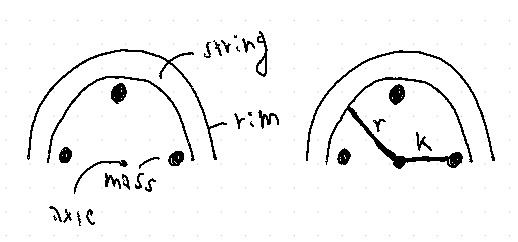
\includegraphics[width=2.3in]{graphics/rAndK.png}
	\end{figure}

	\begin{figure}
		\caption{\rwheel~Inertia Wheel Apparatus
		\label{fig:apparatus}
		\cite{labManual}}
		\centering
		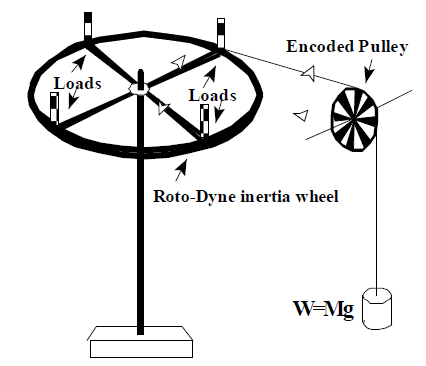
\includegraphics[width=2in]{graphics/apparatus.png}
	\end{figure}

	\subsection{Taking Measurements}
	
	\paragraph{Preliminary Measurements}
	Before conducting our experiment, we took measurements of various parts of our setup. First we obtained $r$ from the lab manual, the distance from the axle of the wheel to the string, and then we measured $k$, the distance from the axle of the wheel to the masses. Our measurement for $k$ was originally $0.073$, but we shifted it to $0.173$ because the original value did not make sense given the radius. After careful deliberations we are very certain it was the result of misreading the ruler, but have used a fairly large uncertainty interval for $k$, $0.01 \text{m}$, as a result of this. For $r$ we used the provided uncertainty of $\pm 0.002 \text{m}$.
	
	\begin{align}
		r&=0.200 \pm 0.002\ \text{m} \label{eq:def-r} \\
		k&=0.173 \pm 0.01\ \text{m} \label{eq:def-k}
	\end{align}

	We used a counterweight with a given mass of $0.06\text{kg}$ to provide a torque to spin our \rwheel, as can be seen in figure~\ref{fig:apparatus}. To account for friction, we incrementally added paperclips to the bottom of the counterweight. We continued to add paperclips up until the mass would fall at a constant speed to counteract the force of friction, using \loggerpro~software and an encoded pulley to monitor acceleration and velocity during this process. Let $M_c$ be the mass of the counterweight and $M_p$ be the mass of the paperclips opposing friction, not used in our computations but still important to the experimental design and recorded below.
	
	\begin{align}
		M_p&=0.0015 \pm 0.0001\ \text{kg} \label{eq:def-mp} \\
		M_c&=0.06\ \text{kg} \label{eq:def-mc}
	\end{align}

	Also, we were provided with the mass of the \rwheel, $M_R$ and the mass loads, $M_L$, of which there were 4.
	
	\begin{align}
		M_R &= 1.5\ \text{kg} \label{eq:def-mr} \\
		M_L &= 0.225 \pm 0.002\ \text{kg} \label{eq:def-ml}
	\end{align}
	
	For the encoded pulley that we used to measure velocity and length of unrolled string it was given that the gaps between intervals of measurement, $\Delta{s}$, was
	
	\begin{align}
		\Delta{s}=0.015\ \text{m}
	\end{align}

	\subsection{Rough Estimation of $I_1$} \label{sect:estimating-moment-of-inertia}

	Before measuring the moment of inertia, we decided to make a rough approximation. To do this, we used two different formulas from common models for moments of inertia, the moment of inertia of a disc, $\frac{1}{2}Mr^2$, and the moment of inertia of a ring, $Mr^2$. These computations will not be accurate since the actual Rote-Dyne disc is neither a perfect disc nor a hoop, and it does not have uniform density even if it were. For our rough estimates, we took the radius to be $r$, and the mass to be
	
	\begin{align}
		M_{tot}&=M_R + 4 M_L \notag \\
		&= 2.4\ \text{kg}
	\end{align}
	
	For the disc estimate, we got
	
	\begin{align}
		I_{\text{disc}}&=\frac{1}{2}Mr^2 \notag \\
		&= 0.048\ \iUnit
	\end{align}
	
	For the hoop estimate, we got
	
	\begin{align}
		I_{\text{hoop}}&= Mr^2 \notag \\
		&= 0.096\ \iUnit
	\end{align}

	To determine an overall estimate, $I_{\text{est}}$, we averaged $I_{\text{disc}}$ and $I_{\text{hoop}}$, and then set the uncertainty to be that average. Assuming that the wheel is a hoop is an under-estimate, and assuming that the wheel is a disc is an over-estimate, the actual moment of inertia should be somewhere between the two.
	
	\begin{align}
		I_{\text{est}}&=\frac{I_{\text{disc}} + I_{\text{hoop}}}{2} \notag \\
		&= 0.072 \pm 0.072\ \iUnit \label{eq:def-i-est}
	\end{align}

	\subsection{Monte Carlo Simulation}
	
	Before actually measuring the moment of inertia, we performed a Monte Carlo Simulation using our estimated $I$ so that we could compare a graph of data of the estimated value to a graph of data for the actual value later on. This simulation involves pretending that our estimated value for $I_1$, $I_{1, \text{est}}$, is the value for $I_1$, and then artificially inducing uncertainty with simulated randomness.
	
	To perform this simulation, we began by creating a new \origin~document, and arranged a table including a column for $\Delta{s}$, the overall displacement (vertical distance it has fallen) of the string, and $\Delta{T_0}$, the time elapsed since dropping the counterweight to arrive at that overall displacement. The values for $\Delta{s}$ were computed using the equation
	
	\begin{align}
		y_i=i \Delta{s}
	\end{align}

	Which is simply stating that the total displacement of the rope is equal to the amount of a single displacement, a notch in the encoded pulley, times the number of increments, which is the total number of notches that passed by the laser at a given time point. To compute the $\Delta{T_0}$ from the $\Delta{s}$ we derived the following equation from equations \ref{eq:delta-s-delta-t} and \ref{eq:conservation-of-energy-gy-form}.
	
	First, we manipulated equation \ref{eq:conservation-of-energy-gy-form} by solving for $v$.
	
	\begin{align}
		gy&=\frac{1}{2}(1 + \frac{I}{Mr^2}) \cdot v^2 \notag \\
		v^2&=\frac{\frac{1}{2}(1 + \frac{I}{Mr^2})}{gy} \notag \\
		v&=\sqrt{\frac{\frac{1}{2}(1 + \frac{I}{Mr^2})}{gy}} \label{eq:equation-for-v}
	\end{align}
	
	Next we solved equation \ref{eq:delta-s-delta-t} for t. For our use case here, we will allow $\Delta{T}$ to be $\Delta{T_0}$. $\Delta{T_0}$ is simply the amount of time elapsed since dropping the counterweight (or, in this case, since the start of the point at which a counterweight would have been dropped, since this is a simulation).
	
	\begin{align}
		v&\approx \frac{\Delta{s}}{\Delta{T}} \tag{\ref{eq:delta-s-delta-t}} \\
		\Delta{T}&\approx \frac{\Delta{s}}{v} \notag \\
		\Delta{T_0}&= \frac{\Delta{s}}{v} \label{eq:equation-for-delta-t-0}
	\end{align}
	
	Then, we solved for $\Delta{T_0}$ by plugging in $v$ from equation~\ref{eq:equation-for-delta-t-0} and $\Delta{s}$ into equation~\ref{eq:equation-for-delta-t-0}.
	
	\begin{align}
		\Delta{T_0}&= \frac{\Delta{s}}{v} \notag \\
		\Delta{T_0}&= \frac{\Delta{s}}{\sqrt{\frac{\frac{1}{2}(1 + \frac{I}{Mr^2})}{gy}}} \notag \\
		\Delta{T_0}^2&= \frac{\Delta{s}^2}{\frac{\frac{1}{2}(1 + \frac{I}{Mr^2})}{gy}} \notag \\
		\Delta{T_0}^2&= \frac{\Delta{s}^2 (1 + \frac{I}{M r^2})}{2gy} \notag \\
		\Delta{T_0}&= \Delta{S} \sqrt{\frac{(1 + \frac{I}{M r^2})}{2gy}}
	\end{align}

	With a simple script we had \origin~apply this equation to each row, utilizing that respective row's $\Delta{s}$ value. Now, since this data is purely based on an estimated moment of inertia value, we applied Monte Carlo randomization. To do this, we shifted each $\Delta{T0_i}$ by some $\Delta{T0_Gi}$ obtained from a Gaussian distribution $G$ with the given mean $0$ and $\sigma$ equal to the estimated uncertainty for $\Delta{t}$, $\delta_{\Delta{t}}$, which was given to be $0.0002 \text{s}$, resulting with a column with values for $\delta{t_R}$. This process can be expressed formulaically as
	
	\begin{align}
		\delta{T_R} = \Delta{T0} + \Delta{t} \cdot \text{grnd}()
	\end{align}

	After running this computation, for the first three values of $\Delta{T_r}$ we got

	\begin{table}[h]
		\centering
		\caption{Samples of random Monte Carlo data generation with seed \texttt{1016}.}
		\begin{tabular}{c|c}
			trial \# & s (m) \\ \hline
			1 & 0.15409 \\
			2 & 0.10925 \\
			3 & 0.08891 \\ \hline
			1 & 0.15381 \\
			2 & 0.10883 \\
			3 & 0.08919 \\ \hline
			1 & 0.01540 \\
			2 & 0.10891 \\
			3 & 0.08891 \\ \hline
			1 & 0.15385 \\
			2 & 0.10918 \\
			3 & 0.08894 \\
		\end{tabular}
	\end{table}
	
	\section{Results}
	
	\begin{figure}[h]
		\centering
		\caption{Monte Carlo Simulation of Rotational Kinetic Energy Experiment plot}
		\label{fig:monte-carlo-simulation}
		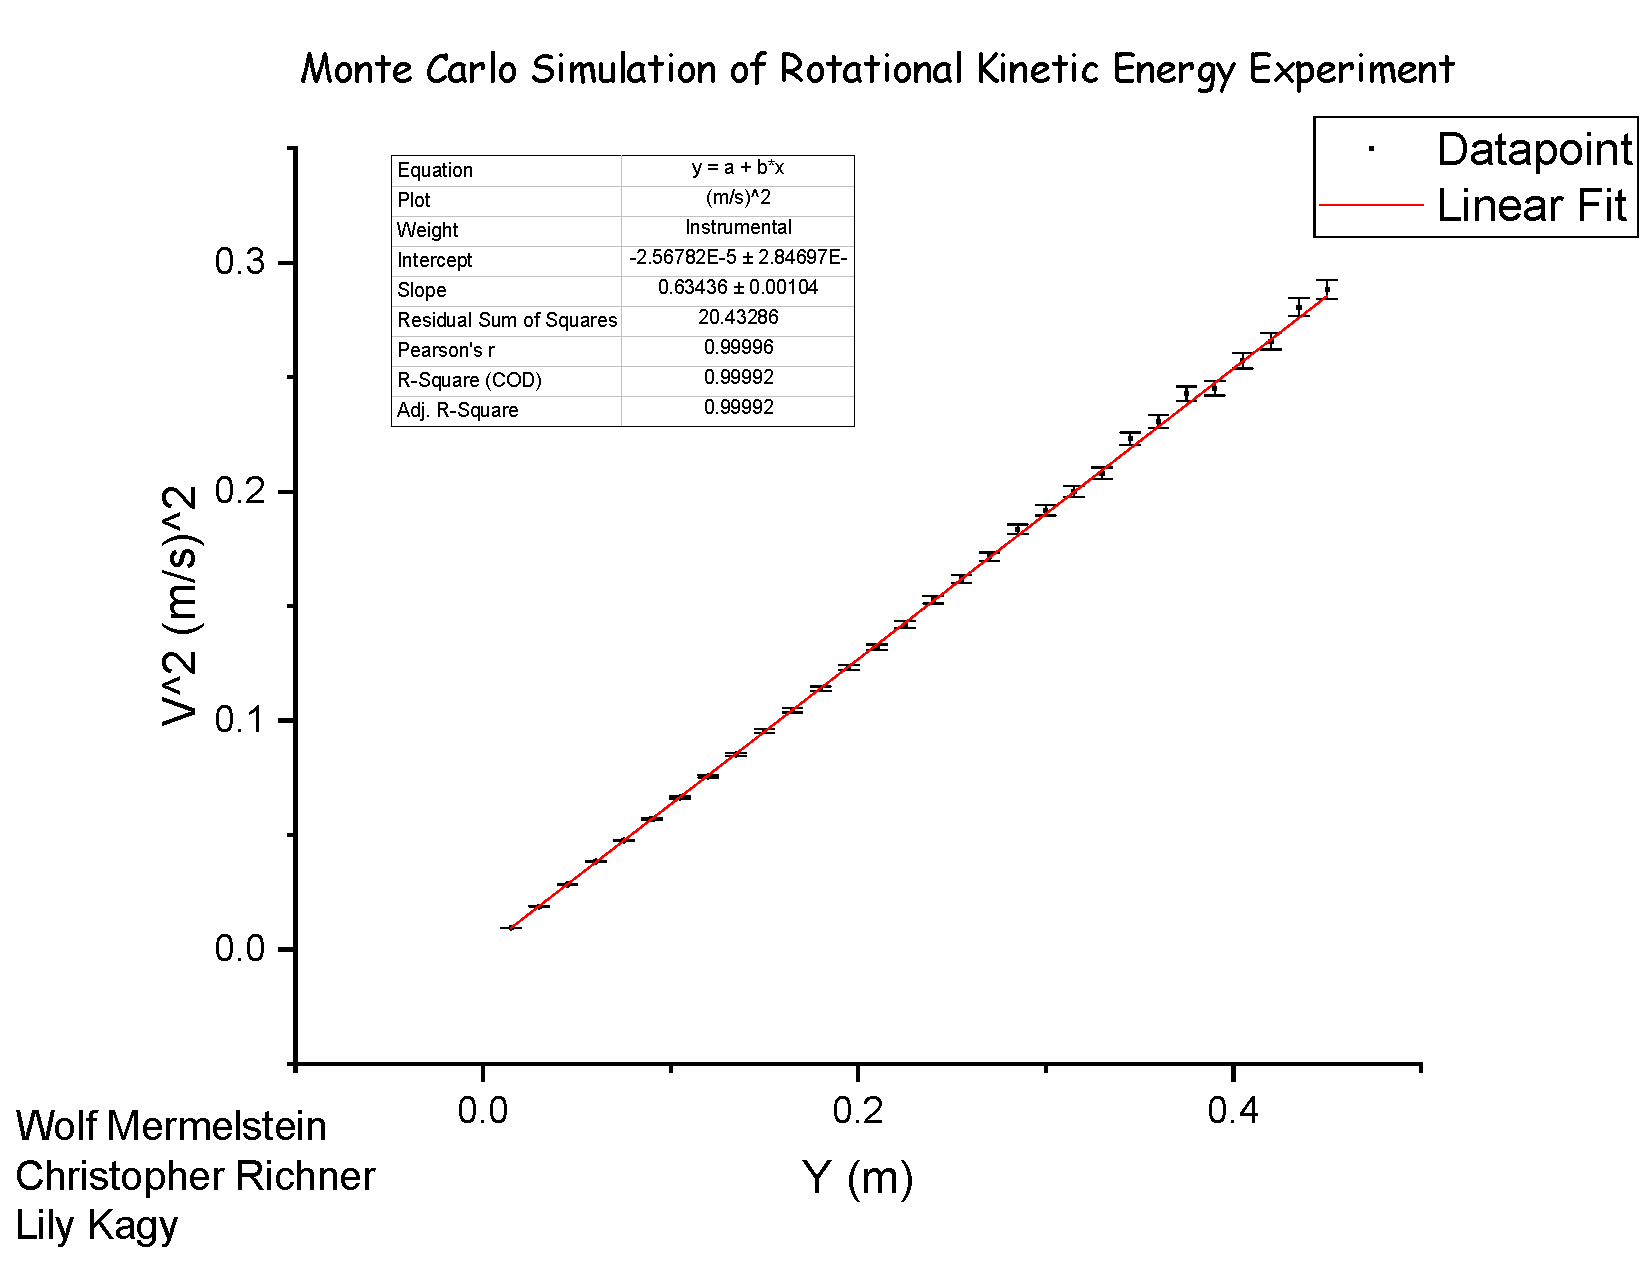
\includegraphics[width=.5\textwidth]{plots/monteCarloPlot.pdf}
	\end{figure}
	
	\begin{figure}[h]
		\centering
		\caption{Without masses $v^2$ vs sDist plot}
		\label{fig:plot-without-masses}
		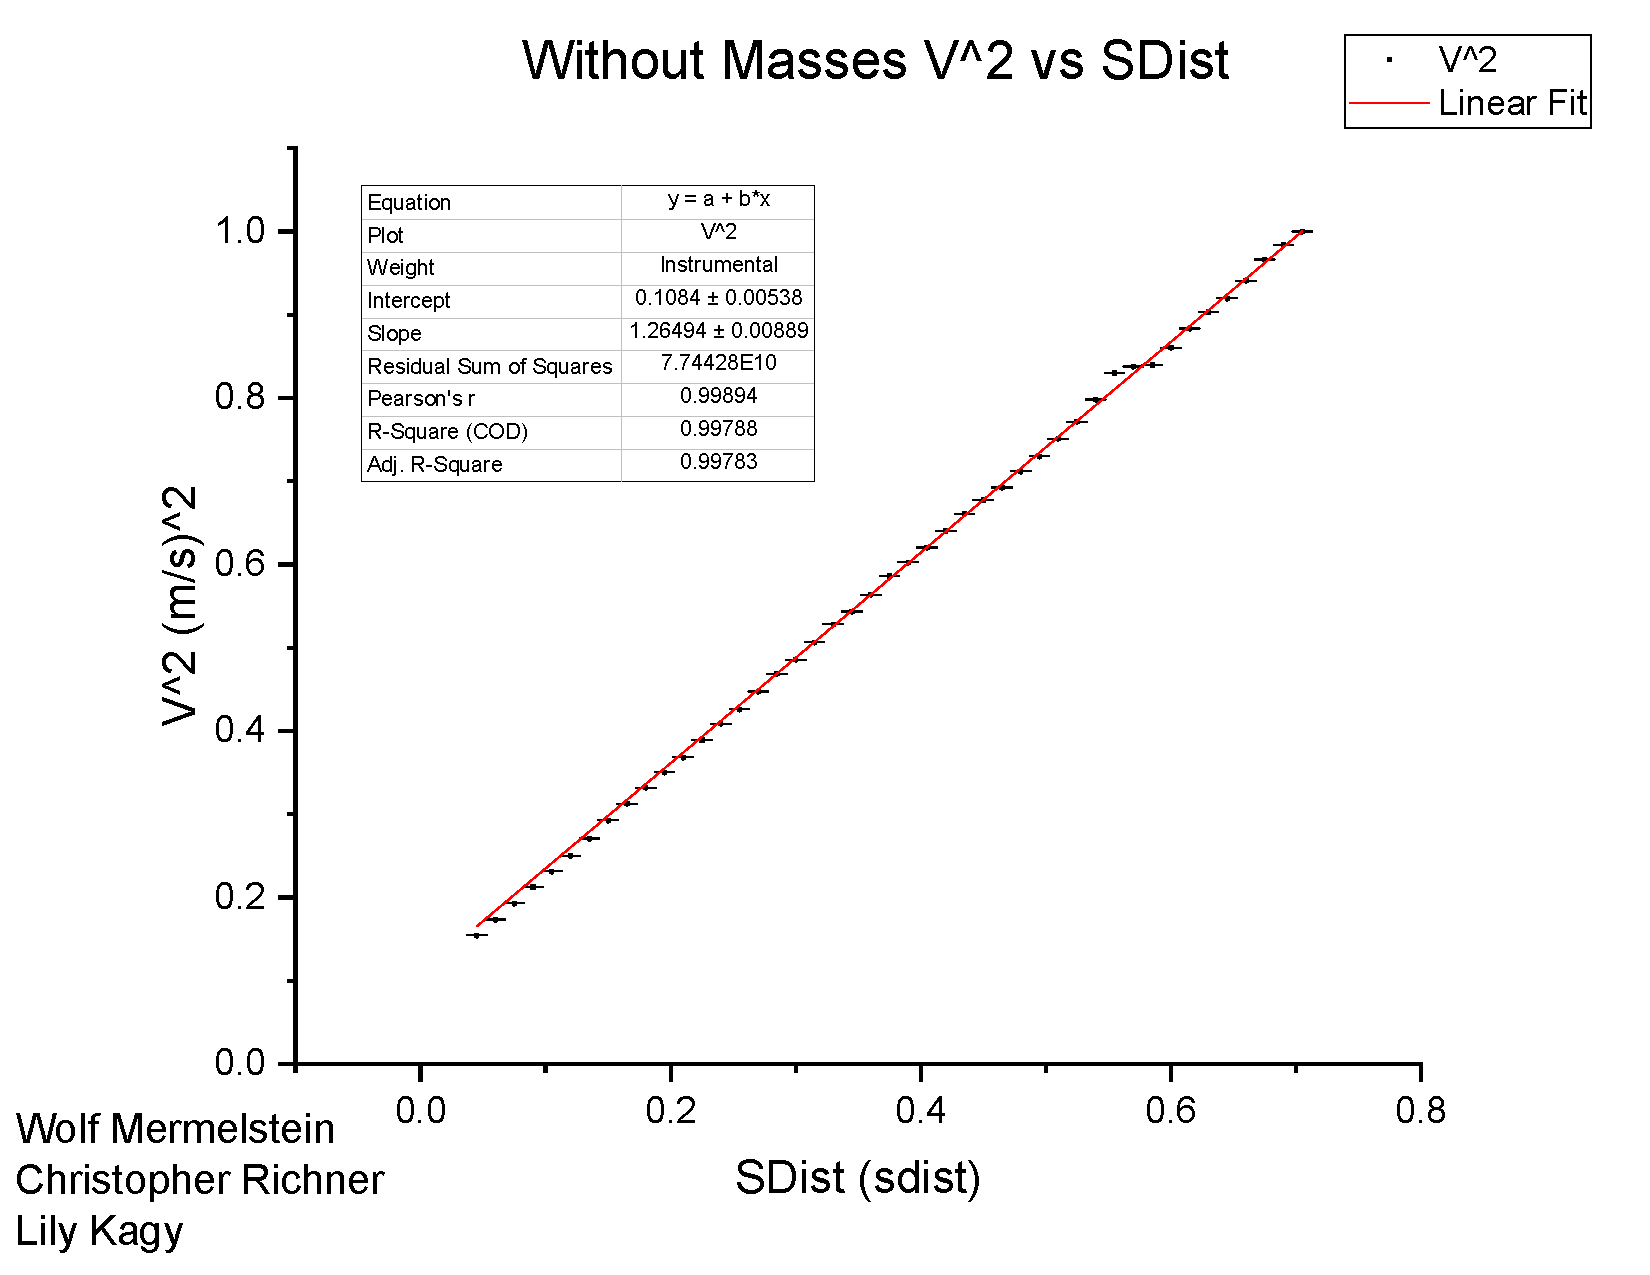
\includegraphics[width=.5\textwidth]{plots/withMassesPlot.pdf}
	\end{figure}

	\begin{figure}[h]
		\centering
		\caption{Masses $v^2$ vs sDist plot}
		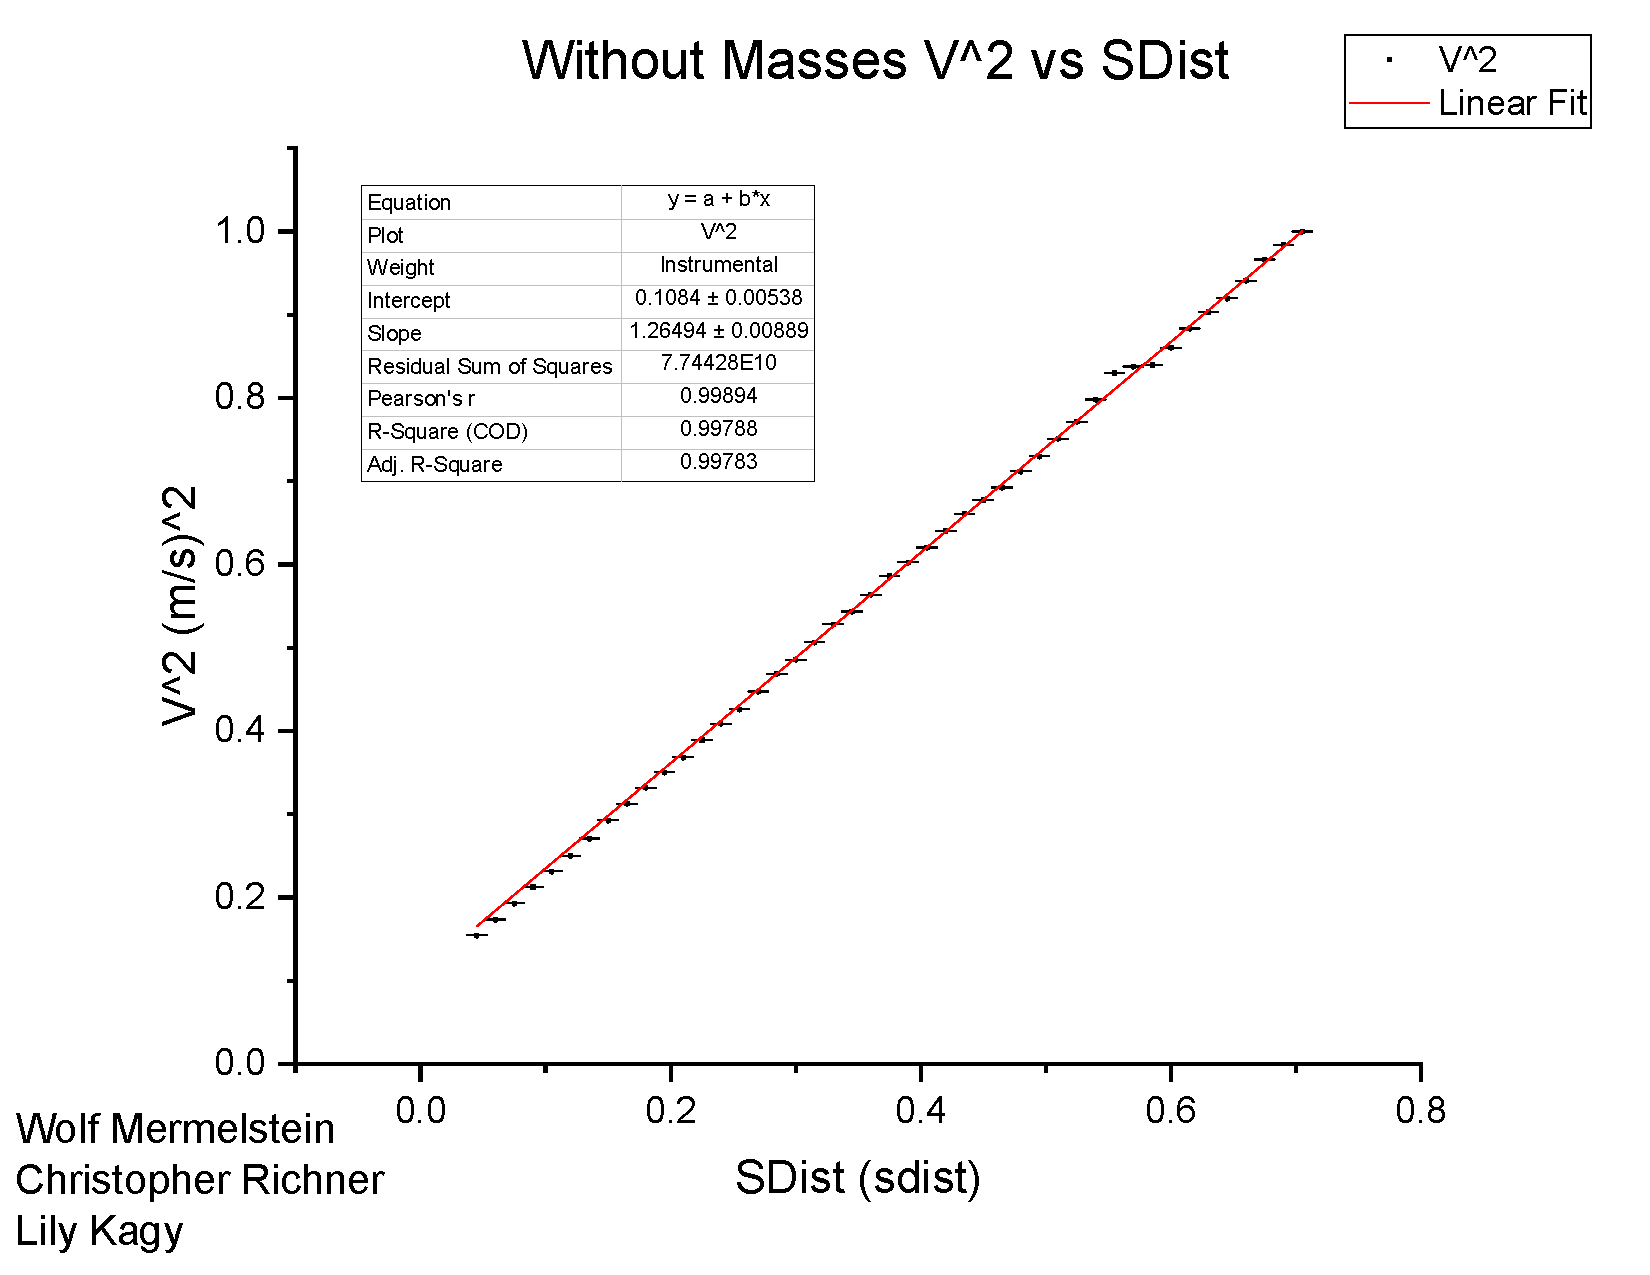
\includegraphics[width=.5\textwidth]{plots/withMassesPlot.pdf}
	\end{figure}
	
	\subsection{Plotting Data}
	
	For the actual results, we measured the velocity,  acceleration, time (duration), and position of the falling counterweight mass using the encoded pulley and \loggerpro. We then imported the data into \origin~for analysis and to help us compile plots. To keep our data consistent, we decided to trim the first three rows and all rows after row 44. Data beyond that in either direction was problematic because of us abruptly setting up and stopping the counterweight from hitting the floor.
	
	To visualize our data, we plotted $v^2$ against displacement for both the system with and without load masses, and did the same for our simulation. For our $v^2$ column in \origin~we used
	
	\begin{align}
		v&=\frac{\Delta{s}}{\Delta{T}} \notag \\
		v^2&=(\frac{\Delta{s}}{\Delta{T}})^2 \notag \\
		v^2&=(\frac{0.015}{\Delta{T}_i})^2 \label{eq:vsqr-base-equation}
	\end{align}

	To include error bars in our \origin~plot, we applied the derivative method row-wise to equation~\ref{eq:vsqr-base-equation}, using equation \ref{eq:vsqr-uncert}. We obtained the value
	
	\begin{align}
		\delta_{\Delta{T}} = 0.0002 \text{s}
	\end{align}

	from our lab manual, which is a consequence of the intrinsic inaccuracy of \loggerpro~and our recording hardware. Solving for $\delta_{v^2}$, we got
	 
	\begin{align}
		\delta_{v^2}&=|\frac{\partial}{\partial \Delta{T_i}} ((\frac{0.015}{\Delta{T}_i})^2) \cdot \delta_{\Delta{t}}| \notag \\
		&=|0.015^2 \cdot \frac{\partial}{\partial \Delta{T_i}} (\Delta{T}^2) \cdot \delta_{\Delta{t}}| \notag \\
		&=|0.000225 \cdot -2 \Delta{T}^{-3} \cdot \delta_{\Delta{t}}| \notag \\
		&=\frac{.00000009}{\Delta{T}^3}
		\label{eq:vsqr-uncert}
	\end{align}
	
	Then we used \origin~to compute a line of best fit, of which the regression and slope has been superposed onto our plot figures, figure \ref{fig:monte-carlo-simulation}, \ref{fig:plot-with-masses}, and \ref{fig:plot-without-masses}.
	
	These aforementioned plots can be found in the appendix, section \ref{sect:appendix}. Additionally, tables \ref{table:with-masses-table} and \ref{table:without-masses-table} contain the actual datatables with raw \loggerpro~data used for generating the plots.
	
	\section{Analysis}
	
	\paragraph{Objective}
	
	For the analysis of our data, our objective was to compute $I_E$, the measured moment of inertia for just the mass loads on the wheel. In order to do this, we took many intermediate steps to prevent mistakes and measurements. This included the previously discussed Monte Carlo simulation process to verify our computation for $I_1$, the moment of the \rwheel~including the mass loads, and an careful estimate of $I_E$ using the definition of moment of inertia for point masses.
	
	\subsection{Computing $I_M$ (Monte Carlo)}
	
	Before examining our experimental values we decided to compute the moment of inertia resultant from our Monte Carlo system. The idea behind this is that for the Monte Carlo system we used our estimated value for $I$, ran a simulation, and applied a randomized skew to the data, so that when computing $I_1$, the moment of inertia for the system with masses, we would have a point of value to compare to.

	Computing $I_M$, the moment of inertia for the Monte Carlo system, and the corresponding $\delta_{I_M}$, the uncertainty in $I_M$ is fairly simple, using equations \ref{eq:i-equation} and \ref{eq:delta-i-formula} for the respective uncertainty.
	
	For the Monte Carlo system, according to our \origin~linear regression model,
	
	\begin{align}
		B_M &= 0.63436 \pm 0.00889\ \mpssq
	\end{align}
	
	We will also henceforth use the generally accepted near-earth gravitational acceleration constant value
	
	\begin{align}
		g &= 9.81 \pm 0.01\ \text{m} \text{s}^2 \label{eq:def-g}
	\end{align}
	
	Plugging in this and other aforestated values into equations \ref{eq:delta-i-formula} and \ref{eq:i-equation}, we get
	
	\begin{align}
		I_M &= Mr^2 \cdot (\frac{2g}{B} - 1) \pm 2 \delta_B \frac{M g r^2}{B^2} \notag \\
		&= 0.07182 \pm 0.00104\ \mpssq
	\end{align}

	In the next section we will use this to determine whether our value $I_1$, the moment of inertia for the system with masses, is reasonable
	
	\subsection{Computing $I_1$ (w/masses)}
	
	The first step towards accomplishing this goal was to determine whether our estimate for the moment of inertia of the \rwheel~was reasonably close to our measured moment value. In order to make this determination we first worked to derive a formula for $I$, the measured value of the moment of inertia. To start, we note the equation for the slope of the \rwheel~with the load masses, $B_1$ and $B_2$, the slope without load masses, obtained through \origin's provided linear fit line.

	\newcommand{\massSlopeUncert}{\delta_B}

	\paragraph{Solving for $I_1$}
	
	Using the same equations that we used in the Monte Carlo simluation, \ref{eq:i-equation} and \ref{eq:delta-i-formula}, we then solved for $I_1$ for the system including the load masses. Most of the values have already been discussed earlier in our procedure. The two novel values are $B_1$ and its uncertainty, $\delta_B$.
	
	\begin{align}
		B_1 &= 0.68204 \pm 0.00168\ \mpssq \label{eq:def-b1}
	\end{align}

	So, applying equations \ref{eq:i-equation}, we get
	
	\begin{align}
		I_1 &= Mr^2 \cdot (\frac{2g}{B} - 1) \pm 2 \delta_B \frac{M g r^2}{B^2} \notag \\
		&= 0.06663 \pm 0.00017\ \iUnit \label{eq:def-i-measured}
	\end{align}

	Looking back at our Monte Carlo value for $I$, $I_M$ and placing it inline with our measured value, we have
		
	\begin{align}
		I_M &= 0.07182 \pm 0.00104\ \iUnit \notag \\
		I_1 &= 0.06663 \pm 0.00017\ \iUnit \tag{\ref{eq:def-i-measured}}
	\end{align}

	To determine if our measured value falls within two uncertainty intervals of our Monte Carlo value, we first determine the distance of a double uncertainty interval to be
	 
	\begin{align}
		\delta_{I_1} \cdot 2 \notag \\
		&= 0.00017 \cdot 2 \notag \\
		&= 0.00034 \notag
	\end{align}
	
	So, mathematically, we are checking
	
	\begin{align}
		0.06663 &\notin \notag \\
		&\notin [0.07182 - 0.00034, 0.07182 + 0.00034] \notag \\
		&\notin [0.07148, 0.07216]
	\end{align}

	\newcommand{\iSkew}{\Delta{I}_{\text{skew}}}

	Which is false, so our measured indeed value \textbf{does not} fall within one to two uncertainty intervals from our estimate. It is, however, close enough that we do not believe that we completely screwed up. The value makes sense; our approximations are just unideal.

	\subsection{Computing $I_2$ (w/o masses)}
	
	\paragraph{Solving for $I_2$}
	
	Next we compute the value of $I_2$, the moment of inertia of the \rwheel~without mass loads, using the same equations for $I_1$, equation \ref{eq:i-equation} and for $\delta_{I_2}$, equation \ref{eq:delta-i-formula}.
	
	For the system without masses, \origin~produced the linear regression value
	
	\begin{align}
		B_2 = 1.26494 \pm 0.00889\ \mpssq \label{eq:def-b2}
	\end{align}
	
	So, plugging our values into equations \ref{eq:i-equation}~and \ref{eq:delta-i-formula}, we get
	
	\begin{align}
		I_2 &= Mr^2 \cdot (\frac{2g}{B} - 1) \pm 2 \delta_B \frac{M g r^2}{B^2} \notag \\
		&= 0.03482 \pm 0.00026\ \iUnit
	\end{align}

	for the massless system. It makes intuitive sense that the moment of inertia is lesser. Inertia is a measure of all the infinite infinitesimally small point masses of an object. There are less masses in the system without mass loads, so the moment of inertia indeed should be notably lesser.
	
	\subsection{Computing $I_E$ (mass loads)}
	
	We are now very close to being able to find $I_E$, the moment of just the mass loads. Knowing the experimental moment of inertia for the system with the mass loads and the system without the mass loads, we can compute $I_E$ by subtracting the moment of inertia of the system with the mass loads by the system without the mass loads.
	
	\begin{align}
		I_E &= I_1 - I_2 \label{eq:mass-load-i-only} \\
		&= 0.06663 - 0.03482 \notag \\
		&= 0.03181\ \iUnit
	\end{align}
	
	We will base the uncertainty of this measurement on the literal, complete equation, subbing $I$ into equation~\ref{eq:mass-load-i-only} for equation \ref{eq:i-equation}.
	
	\begin{align}
		I_E &= I_1 - I_2 \tag{\ref{eq:mass-load-i-only}} \\
		&= M r^2 \cdot (\frac{2g}{B_1} - 1) - Mr^2 \cdot (\frac{2g}{B_2} - 1) \notag \\
		&= M r^2 ((\frac{2g}{B_1} - 1) - (\frac{2g}{B_2} - 1)) \notag \\
		&= M r^2 \frac{2g(B_2 - B_1)}{B_1 B_2}
	\end{align}

	Writing the equation like this does not help us solve for $I_E$, in fact if anything it makes it more convoluted. Rather, the purpose of this literal expression is to allow us to compute an uncertainty based on the values that it is based on. We believe that $\delta_{I_E, M}$ and $\delta_{I_E, g}$ are negligible in comparison to $\delta_{I_E, r}$, $\delta_{I_E, B_1}$, and $\delta_{I_E, B_2}$, since, besides the fact that the actual value for $\delta_M$ is $0.0001 \text{kg}$, $r$ is squared which makes its uncertainty even more significant. To start, we recall
	
	\begin{align}
		B_1 &= 0.68204 \pm 0.00168\ \mpssq \tag{\ref{eq:def-b1}} \\
		B_2 &= 1.26494 \pm 0.00889\ \mpssq \tag{\ref{eq:def-b2}} \\
		r &= 0.200 \pm 0.002\ \text{m} \tag{\ref{eq:def-r}} \\
		M &= 0.0600 \pm 0.0001\ \text{kg} \tag{\ref{eq:def-mc}} \notag \\
		g &= 9.81 \pm 0.01 \frac{m}{\text{s}^2} \tag{\ref{eq:def-g}}
	\end{align}
	
	To compute the overall uncertainty $\delta_{I_E}$, we will first compute $\delta_{I_E, r}$ using the derivative method, and $\delta_{I_E, B_1}$, and $\delta_{I_E, B_2}$ using the computational method, and then will add all the uncertainties in quadrature.
	
	\begin{align}
		\delta_{I_E, r} &= |\frac{\partial}{\partial r}(M r^2 \frac{2g(B_2 - B_1)}{B_1 B_2}) \cdot \delta_r| \notag \\
		&= |2r M \frac{2g(B_2 - B_1)}{B_1 B_2} \cdot \delta_r| \notag \\
		&\approx 0.00063\ \iUnit
	\end{align}

	\begin{align}
		\delta_{I_E, B_2} &= |M r^2 \frac{2g(B_2 - B_1)}{B_1 B_2} - \notag \\
		&M r^2 \frac{2g((B_2 + \delta_{B_2}) - B_1)}{B_1 (B_2 + \delta_{B_2})}| \notag \\
		&\approx 0.00026\ \iUnit
	\end{align}

	\begin{align}
		\delta_{I_E, B_1} &= |M r^2 \frac{2g(B_2 - B_1)}{B_1 B_2} - \notag \\
		&M r^2 \frac{2g((B_1 + \delta_{B_1}) - B_1)}{(B_1 + \delta_{B_1}) B_2}| \notag \\
		&\approx 0.00017\ \iUnit
	\end{align}

	So, to find the overall uncertainty we add in quadrature, getting
	
	\begin{align}
		\delta_{I_E} &= \\
		&= \sqrt{\delta_{I_E, r}^2 + \delta_{I_E, B_1}^2 + \delta_{I_E, B_2}^2} \notag \\
		&= \sqrt{0.00063^2 + 0.00026^2 + 0.00017^2} \notag \\
		&\approx 0.00070\ \iUnit
	\end{align}

	We can then succinctly state that
	
	\begin{align}
		I_E = 0.03181 \pm 0.00070\ \iUnit \label{eq:def-ie}
	\end{align}

	\subsubsection{Estimating $I_E$}
	
	Now, like how we came up with an approximate value for the \rwheel~with masses and loads by approximating it to be a disc and a ring and averaging the two, we wanted to come up with a estimate in similar fashion for $I_E$. To do this, we treated the four loads $M_L$, of $0.225 \pm 0.002 \text{kg}$ each, as point masses for computing an estimate for $I_E$. To do this, we applied equation \ref{eq:def-i} to all 4 point masses. Note that we use $k$ here instead of $r$ since the masses are at distance $k$ from the center of the \rwheel.
	
	\begin{align}
		I_{\text{est}, E} &= \sum{M k^2} \notag \\
		&= 4 (M_L k^2) \notag \\
		&= 4 \cdot 0.225 \cdot 0.173^2 \notag \\
		&= 0.02693\ \iUnit
	\end{align}
	
	Computing $\delta_{I_{\text{est}, E}}$ is fairly trivial, requiring us to propagate $\delta_k$ and $\delta_{M_L}$'s effect on $\delta_{I_{\text{est}, E}}$ and then sum in quadrature. For this we used the derivative method.
	
	\begin{align}
		\delta_{I_{\text{est}, E}, k} \notag \\
		&= |\frac{\partial}{\partial k} (4 (M_L k^2)) \cdot \delta_k| \notag \\
		&= |8 M_L k \delta_k| \notag \\
		&= |8 \cdot 0.225 \cdot 0.173 \cdot 0.01| \notag \\
		&\approx 0.00311\ \iUnit
	\end{align}
	
	\begin{align}
		\delta_{I_{\text{est}, E}, M_L} \notag \\
		&= |\frac{\partial}{\partial M_L} (4 M_L k^2 \delta_{M_L})| \notag \\
		&= |4 k^2 \delta_{M_L}| \notag \\
		&= |4 \cdot 0.173^2 \cdot 0.002| \notag \\
		&\approx 0.00023\ \iUnit
	\end{align}
	
	Adding the uncertainties $\delta_{I_{\text{est}, E}, M_L}$ and $\delta_{I_{\text{est}, E}, r}$ in quadrature we get
	
	\begin{align}
		\delta_{I_{\text{est}, E}} &= \sqrt{\delta_{I_{\text{est}, E}, r}^2 + \delta_{I_{\text{est}, E}, M_L}^2} \notag \\
		&= \sqrt{0.00311^2 + 0.00023^2} \notag \\
		&\approx 0.00311\ \iUnit
	\end{align}

	Succinctly, we can thus state
	
	\begin{align}
		I_{\text{est}, E} = 0.02693 \pm 0.00311\ \iUnit
	\end{align}

	Now we can compare this to our value for $I_E$ to see if it is reasonable and agrees two within two uncertainty intervals. We recall that our value for $I_E$ is
	
	\begin{align}
		I_E = 0.03181 \pm 0.00070\ \iUnit \tag{\ref{eq:def-ie}}
	\end{align} 

	Two uncertainty intervals from $I_E$ is
	
	\begin{align}
		\delta_{I_E} \cdot 2 \notag \\
		=& 0.00311 \cdot 2 \notag \\
		=& 0.00622
	\end{align}

	So, upon inspection of the mathematical statement
	
	\begin{align}
		0.02693 \in [0.03181 - 0.00622, 0.03181 + 0.00622] \notag \\
		0.02693 \in [0.02559, 0.03803] \notag \\
	\end{align}

	we determine that indeed our estimated uncertainty lies within two uncertainty intervals. This provides us assurance that our value for $I_E$ is indeed reasonable. 
	
	What we have shown is that estimates for point masses seem to be more reliable than estimates based off of disc or ring approximations for \rwheel s.
	
	\section{Conclusion}
	
	Ultimately, using the law of conservation of angular momentum we were able to show that moments of inertia are able to be experimentally measured. These specific equations that we obtained based on the law of conservation of rotational inertia and the equation that we found for the respective uncertainty are very useful. In certain applications, such as those of objects with nonuniform density or shape, the technique presented proves particularly useful in determining the moment of inertia, since in such cases estimates involving integrals are very difficult and often rely on approximations. 
	
	We also showed that although Monte Carlo simulations are useful in inducing uncertainty in this specific use case, it still greatly hinges on the estimated value for the moment that you use for determining whether the simulated $I_M$ is close to the actual value of $I$. This, we noticed, greatly depends on the specific approximation used. In our case, we found that using disc and hoop approximations for the \rwheel~was much less ideal than the point mass approximations that we used for the load masses in computing moments, which is an interesting and potentially unintuitive finding.
	
	\section*{Acknowledgments}
	I would like to thank Christopher Richner and Lily Kagy, CWRU Department of Physics, for their help in obtaining the experimental data, collaborating on preparation of the figures, and checking calculations. Additionally, I would like to thank Olivia Green, CWRU Department of Physics, for helping facilitate our lab. Also, I would like to thank the authors of our lab manual, which was of great aid in writing this report.
	
	\bibliographystyle{plain}
	\nocite{textbook}
	\nocite{labManual}
	\bibliography{sources}
	
	\onecolumn
	
	\section{Appendix} \label{sect:appendix}
		
	As this lab was compiled with \LaTeX, the resources and files used for the lab are all stored within the same folder as the submission, which is located in a Github repository at \url{https://github.com/404wolf/phys123-lab5-rke}. This appendix contains enlarged plots for our lab, along with the raw data tables obtained from \loggerpro~and used by \origin.
		
	\subsection{Enlarged figures and Datatables}
	
	\begin{figure}[h]
		\centering
		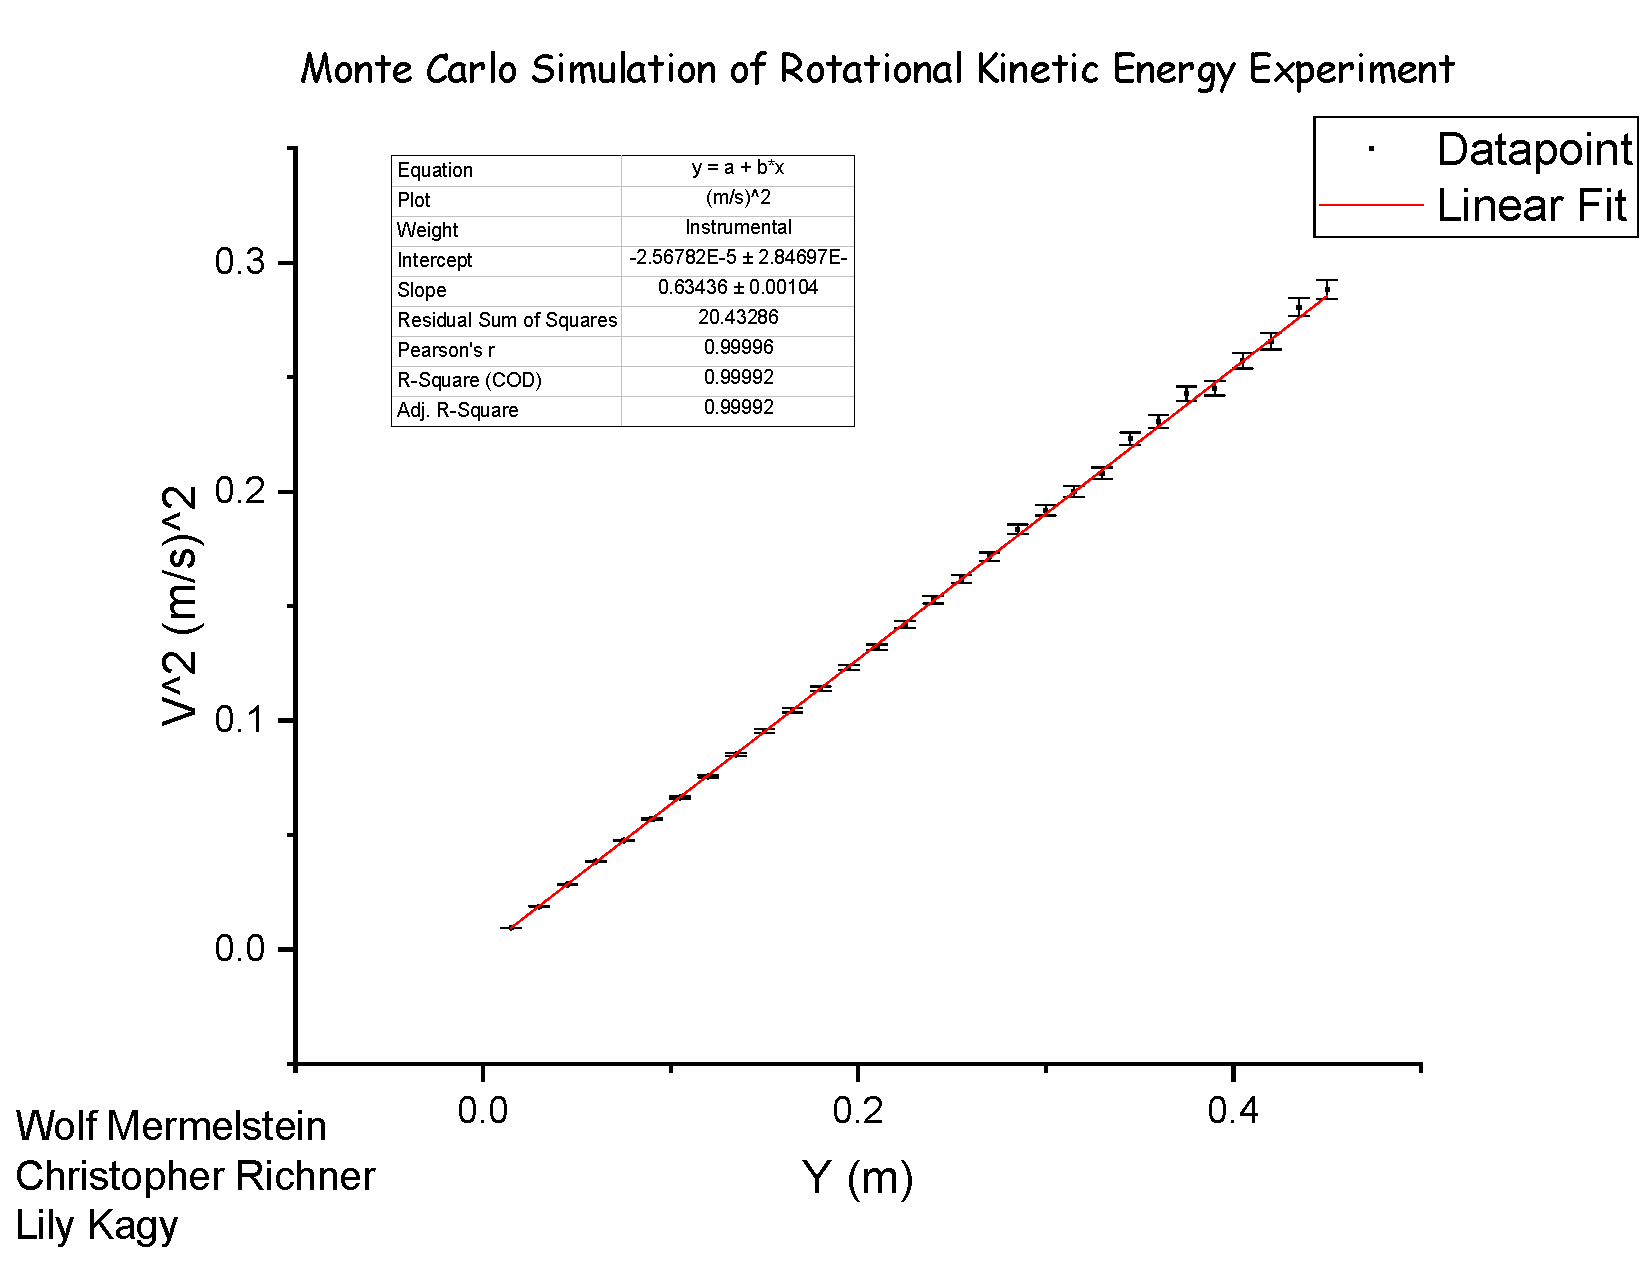
\includegraphics[width=6in]{plots/monteCarloPlot.pdf}
	\end{figure}
		
	\begin{figure}[h]
		\centering
		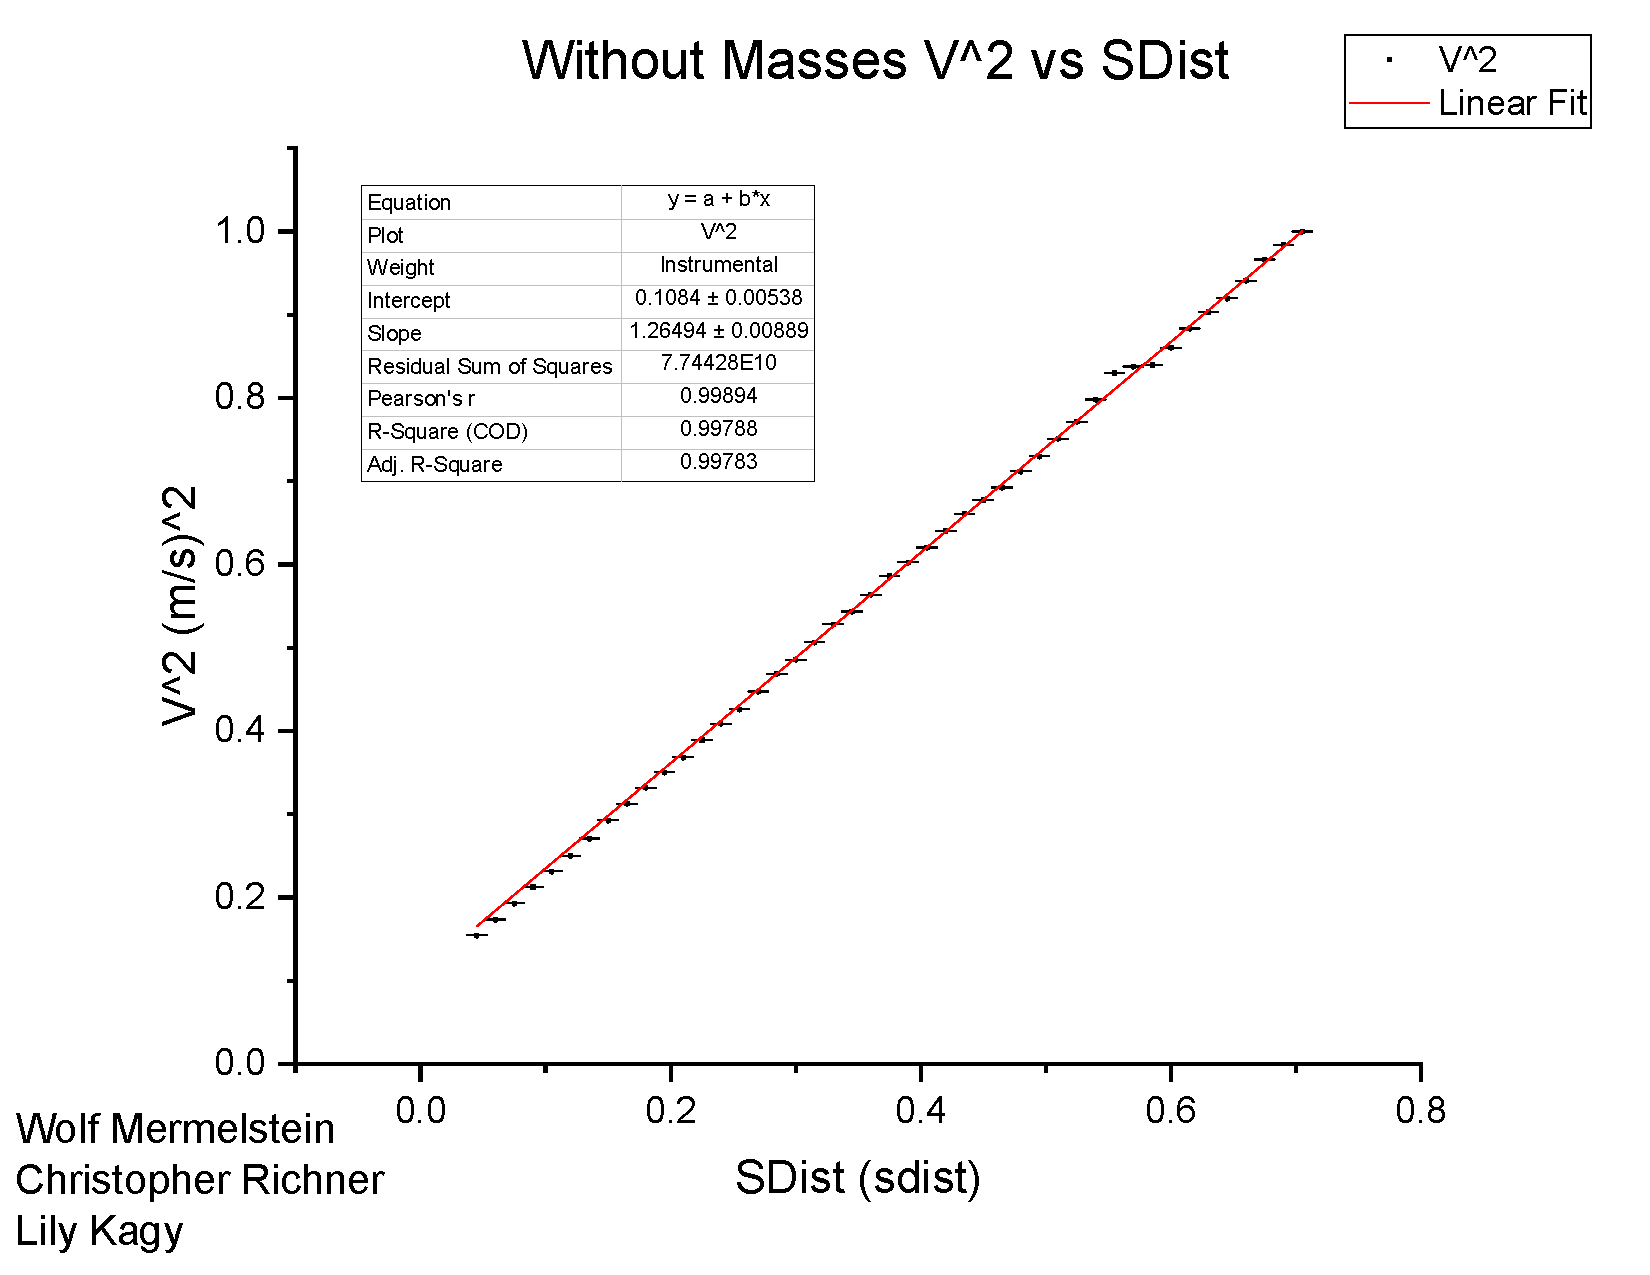
\includegraphics[width=6in]{plots/withMassesPlot.pdf}
	\end{figure}
		
	\begin{figure}[h] 
		\centering
		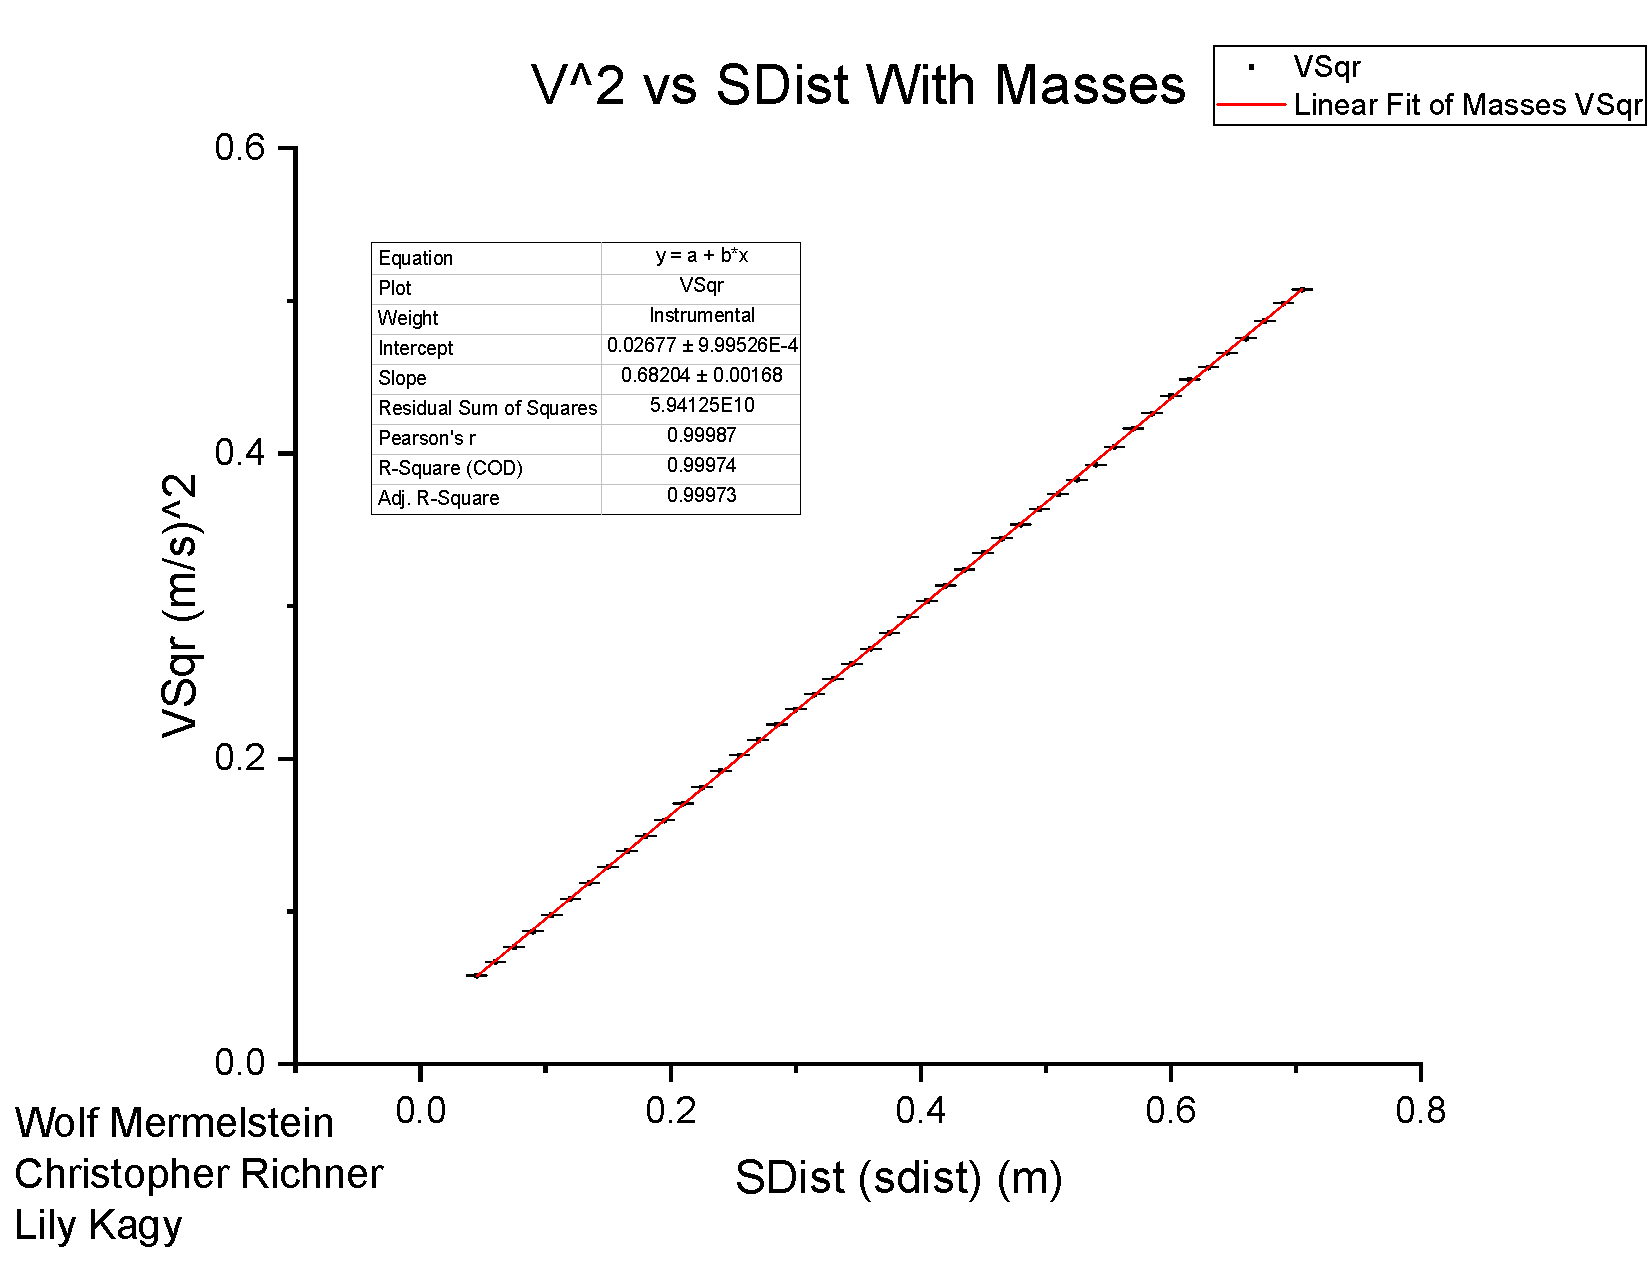
\includegraphics[width=6in]{plots/withoutMassesPlot.pdf}
	\end{figure}
	
	\begin{table}[!ht]
		\caption{Data for falling counterweight \textbf{without} mass loads in place}
		\label{table:without-masses-table}
		\vspace{.1in}
		
		\centering
		\begin{tabular}{|l|l|l|l|l|}
			Time & STime & SDist & SVel & SAccel \\ \hline
			t & stime & sdist & svel & saccel \\ \hline
			s & s & m & m/s & m/s\^2 \\ \hline
			0.2003832 & 0.3409468 & 0.045 & 0.240637469 & 0.2974361002 \\ \hline
			0.2421024 & 0.4010488 & 0.06 & 0.2587705469 & 0.3059740303 \\ \hline
			0.2727832 & 0.4571542 & 0.075 & 0.2768823709 & 0.3396616489 \\ \hline
			0.3099096 & 0.5096392 & 0.09 & 0.2950082819 & 0.3510465914 \\ \hline
			0.3375832 & 0.5590336 & 0.105 & 0.3125067287 & 0.3574728706 \\ \hline
			0.371984 & 0.6057826 & 0.12 & 0.3289729322 & 0.3469787101 \\ \hline
			0.3977972 & 0.6503324 & 0.135 & 0.3445762028 & 0.3535079613 \\ \hline
			0.4301136 & 0.6929332 & 0.15 & 0.3594867431 & 0.3465042602 \\ \hline
			0.4541972 & 0.7338524 & 0.165 & 0.3734799691 & 0.3374400019 \\ \hline
			0.4841948 & 0.7733118 & 0.18 & 0.3866063477 & 0.3278706007 \\ \hline
			0.506816 & 0.8114928 & 0.195 & 0.3997294453 & 0.3595444818 \\ \hline
			0.5350836 & 0.8484054 & 0.21 & 0.4130797945 & 0.3638046842 \\ \hline
			0.5563028 & 0.8841552 & 0.225 & 0.4258449397 & 0.3503333039 \\ \hline
			0.5829836 & 0.9188832 & 0.24 & 0.4381633461 & 0.3590888604 \\ \hline
			0.6031832 & 0.9526498 & 0.255 & 0.4497965385 & 0.3299465981 \\ \hline
			0.6285816 & 0.9856 & 0.27 & 0.4607194593 & 0.3330491259 \\ \hline
			0.6478832 & 1.0177834 & 0.285 & 0.4715773455 & 0.3417015924 \\ \hline
			0.6720832 & 1.0492332 & 0.3 & 0.4820423673 & 0.3238048217 \\ \hline
			0.6905832 & 1.0800322 & 0.315 & 0.492183323 & 0.3347201767 \\ \hline
			0.7137832 & 1.1101992 & 0.33 & 0.5023979233 & 0.3424834134 \\ \hline
			0.7315832 & 1.1397582 & 0.345 & 0.5121068853 & 0.3144374509 \\ \hline
			0.7539216 & 1.1687902 & 0.36 & 0.5216114938 & 0.3403302933 \\ \hline
			0.7710904 & 1.1972824 & 0.375 & 0.5315253346 & 0.355568289 \\ \hline
			0.792702 & 1.2252416 & 0.39 & 0.5413072074 & 0.3441565057 \\ \hline
			0.8092096 & 1.2527124 & 0.405 & 0.5507273167 & 0.3416705778 \\ \hline
			0.8302836 & 1.2797228 & 0.42 & 0.559880448 & 0.3360780896 \\ \hline
			0.8462136 & 1.3063022 & 0.435 & 0.5692255573 & 0.3671062769 \\ \hline
			0.8665272 & 1.3324336 & 0.45 & 0.5787253594 & 0.359973184 \\ \hline
			0.8820832 & 1.358147 & 0.465 & 0.5869743702 & 0.2816386499 \\ \hline
			0.9017832 & 1.383547 & 0.48 & 0.5946036744 & 0.3190939627 \\ \hline
			0.9168836 & 1.4086054 & 0.495 & 0.602973345 & 0.3489192067 \\ \hline
			0.9359832 & 1.4333056 & 0.51 & 0.6110845183 & 0.3078506391 \\ \hline
			0.9506832 & 1.4577022 & 0.525 & 0.6186489591 & 0.3122719003 \\ \hline
			0.9693164 & 1.481802 & 0.54 & 0.6266088147 & 0.3483025149 \\ \hline
			0.983612 & 1.5055832 & 0.555 & 0.6359267169 & 0.4353334838 \\ \hline
			1.0018836 & 1.5289834 & 0.57 & 0.6452122961 & 0.3582989806 \\ \hline
			1.0158992 & 1.5520834 & 0.585 & 0.6529222225 & 0.3092271113 \\ \hline
			1.0336832 & 1.5749334 & 0.6 & 0.661597301 & 0.4500795393 \\ \hline
			1.0474092 & 1.5974336 & 0.615 & 0.669666613 & 0.2671862678 \\ \hline
			1.0647832 & 1.6197336 & 0.63 & 0.6756628186 & 0.27059002 \\ \hline
			1.0782148 & 1.6418362 & 0.645 & 0.6826017458 & 0.3572933224 \\ \hline
			1.0952812 & 1.663686 & 0.66 & 0.6896131877 & 0.2844921273 \\ \hline
			1.1083832 & 1.6853406 & 0.675 & 0.69766979 & 0.4596086524 \\ \hline
			1.1251172 & 1.7066906 & 0.69 & 0.7060389196 & 0.32438475 \\ \hline
			1.1379832 & 1.7278332 & 0.705 & 0.7123894853 & 0.2763517435 \\ \hline
		\end{tabular}
	\end{table}
	
	\begin{table}[!ht]
		\caption{Data for falling counterweight \textbf{without} mass loads in place}
		\label{table:with-masses-table}
		\vspace{.1in}
		
		\centering
		\begin{tabular}{|l|l|l|l|l|}
			Time & STime & SDist & SVel & SAccel \\
			t & stime & sdist & svel & saccel \\ \hline
			s & s & m & m/s & m/s\^2 \\ \hline
			0.0942928 & 0.1784214 & 0.045 & 0.3931293508 & 0.6331416361 \\ \hline
			0.118666 & 0.2154714 & 0.06 & 0.4167682347 & 0.6429114748 \\ \hline
			0.13679 & 0.2505154 & 0.075 & 0.4395279097 & 0.6560084549 \\ \hline
			0.1593652 & 0.2838154 & 0.09 & 0.4611842509 & 0.6446726969 \\ \hline
			0.1763652 & 0.3156328 & 0.105 & 0.4813227422 & 0.6212064342 \\ \hline
			0.1974776 & 0.3461942 & 0.12 & 0.5002408825 & 0.6168350372 \\ \hline
			0.2134652 & 0.375645 & 0.135 & 0.5204425281 & 0.7550560866 \\ \hline
			0.2334652 & 0.403888 & 0.15 & 0.5411476689 & 0.7111579009 \\ \hline
			0.2485668 & 0.4311196 & 0.165 & 0.5590171297 & 0.6012483335 \\ \hline
			0.2675656 & 0.457576 & 0.18 & 0.5759222213 & 0.6767102446 \\ \hline
			0.2819648 & 0.4832344 & 0.195 & 0.5919181069 & 0.5701239701 \\ \hline
			0.3000652 & 0.5082738 & 0.21 & 0.6071150987 & 0.6437223597 \\ \hline
			0.3138984 & 0.5326654 & 0.225 & 0.6238645636 & 0.7296573993 \\ \hline
			0.3312004 & 0.5563802 & 0.24 & 0.6392812271 & 0.5705149372 \\ \hline
			0.3445048 & 0.5796034 & 0.255 & 0.6528166664 & 0.5951675979 \\ \hline
			0.361188 & 0.602345 & 0.27 & 0.668869986 & 0.8166345302 \\ \hline
			0.3740644 & 0.624472 & 0.285 & 0.6847467198 & 0.618420718 \\ \hline
			0.390102 & 0.6461654 & 0.3 & 0.6968292431 & 0.4955147032 \\ \hline
			0.4024884 & 0.6675292 & 0.315 & 0.7117831029 & 0.9044103837 \\ \hline
			0.417674 & 0.6883282 & 0.33 & 0.7267542228 & 0.53518959 \\ \hline
			0.4292784 & 0.7088134 & 0.345 & 0.737173249 & 0.4820351523 \\ \hline
			0.4445652 & 0.7290278 & 0.36 & 0.7508551143 & 0.8716399856 \\ \hline
			0.4560652 & 0.7487786 & 0.375 & 0.7655336953 & 0.6147383898 \\ \hline
			0.4705868 & 0.768221 & 0.39 & 0.7764021555 & 0.5032779268 \\ \hline
			0.4818648 & 0.7874214 & 0.405 & 0.7876149561 & 0.664697796 \\ \hline
			0.495882 & 0.8063156 & 0.42 & 0.8001386413 & 0.6609667181 \\ \hline
			0.5067812 & 0.8249194 & 0.435 & 0.8130346045 & 0.72541275 \\ \hline
			0.5206656 & 0.8432194 & 0.45 & 0.8231695853 & 0.3822354223 \\ \hline
			0.5311832 & 0.8613652 & 0.465 & 0.8321622217 & 0.6089180588 \\ \hline
			0.5446652 & 0.8792732 & 0.48 & 0.8437710657 & 0.6875800459 \\ \hline
			0.554982 & 0.8969236 & 0.495 & 0.8544283269 & 0.520014252 \\ \hline
			0.5680952 & 0.9143864 & 0.51 & 0.8665462466 & 0.8678410374 \\ \hline
			0.5782656 & 0.931549 & 0.525 & 0.8783503608 & 0.5077214323 \\ \hline
			0.5911116 & 0.948543 & 0.54 & 0.8933737653 & 1.260361948 \\ \hline
			0.6010652 & 0.965139 & 0.555 & 0.9110416678 & 0.8688140546 \\ \hline
			0.6135784 & 0.9814764 & 0.57 & 0.915255149 & -0.3530060006 \\ \hline
			0.6232648 & 0.9979174 & 0.585 & 0.9163732773 & 0.4890230607 \\ \hline
			0.6353656 & 1.0142154 & 0.6 & 0.9275233967 & 0.8792576405 \\ \hline
			0.6447648 & 1.0302654 & 0.615 & 0.9399816885 & 0.673177482 \\ \hline
			0.6569652 & 1.046133 & 0.63 & 0.9503827681 & 0.6378058508 \\ \hline
			0.6663652 & 1.0618334 & 0.645 & 0.9590269548 & 0.4633363769 \\ \hline
			0.6780932 & 1.0774156 & 0.66 & 0.9699853551 & 0.9431916229 \\ \hline
			0.6870656 & 1.0927652 & 0.675 & 0.9830297701 & 0.7564507123 \\ \hline
			0.6985632 & 1.1079356 & 0.69 & 0.9919658955 & 0.4216494522 \\ \hline
			0.7075648 & 1.1230088 & 0.705 & 0.999952488 & 0.6380581699 \\ \hline
		\end{tabular}
	\end{table}
	
\end{document}